\section{Introducere}

% Plasează tema proiectului într-un context mai larg şi furnizează anumite informaţii generale pentru cititor (informaţii mai detaliate vor fi furnizate în secţiunea “Fundamentare teoretică”. 

% Introducerea defineşte de asemenea problema de rezolvat, obiectivele proiectului, descrie pe scurt soluţia propusă şi prezintă conţinutul fiecărei secţiuni următoare din raport.

% • Descrieţi contextul temei proiectului şi tendinţele tehnologice legate de această temă;
% • Definiţi domeniul de studiu, explicaţi terminologia de bază şi descrieţi importanţa
% acestui domeniu;
% • Definiţi clar şi în detaliu problema de rezolvat şi obiectivele principale ale proiectului;
% • Descrieţi pe scurt soluţia propusă şi explicaţi modul în care aceasta este diferită de
% (sau superioară faţă de) alte soluţii existente;

% • În ultimul paragraf al introducerii, prezentaţi ceea ce va conţin fiecare din secţiunile
% următoare ale raportului.

% 2 - 3 pagini. 
% Utilizaţi referinţe la literatura de specialitate sub forma unor numere cuprinse între
% paranteze drepte, ca [1] [5].

\subsection{Osciloscopul Digital}

\paragraph{}
{\bf Osciloscopul} este un aparat electornic de masura ce permite vizualizarea formei unui semnal de voltaj in timp. Osciloscopul este folosit pentru a analiza forma de unda descrisa de un semnal repetitiv. Aceasta vizualizare ofera informatii despre perioada semnalului, amplitudinea acestuia, dar si despre modificari in amplitudine sau perioada. O alta intrebuintare a osciloscoapelor este analiza zgomotelor unui semnal. Fiind aparate de masura ce ofera o reprezentare vizuala detaliata a unui semnal, acestea joaca un rol important in analiza si depanarea circuitelor electrice.

\begin{figure}[h]
\centering
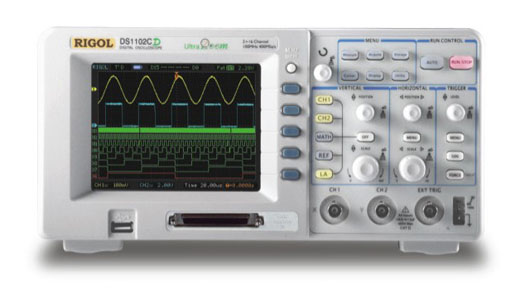
\includegraphics[width=320pt]{digital_oscilloscope}
\caption{Osciloscop Digital}
\label{fig:digital_oscilloscope}
\end{figure}

\paragraph{}
Un osciloscop digital este format din patru componente: un ecran pentru vizualizarea semnalului impreuna cu 3 panori de configuratie ce controleaza dimensiunea amplitudinii semnalului pe monitor, frecventa de esantionare a semnalului, si modul de declansare a esantionarii. Unele osciloscoape digitale ofera posibilitatea masurarii a doua semnale concurent. Aceasta functionalitate este utila daca se urmareste comparatia a doua semnale. De asemenea se pot analiza si semnale digitale daca semnalul analogic de intrare este de asa natura.

\paragraph{}
{\bf Ecranul de vizualizare} este, de cele mai multe ori, un mic monitor CRT integrat in osciloscop. Pe acest monitor se afiseaza semnalul analizat, impreuna cu alte informatii suplimentare cum ar fi o grila de referinta, scala la care este reprezentat semnalul, axele X si Y, sau alti indicatori.

\paragraph{}
{\bf Controlul amplitudinii} este factorul ce determina conversia din valoarea semnalului analogic ( in volti ) in spatiul de afisare al ecranului ( in pixeli ). Folosind acest control putem modifica scala la care este afisat semnalul pe axa Y.

\paragraph{}
{\bf Controlul frecventei de esantionare} ne permite sa modificam frecventa la care osciloscopul citeste semnalul analog. Cu cat frecventa este mai mare, cu atat reconstruirea semnalului pe ecranul de vizualizare este mai fidela. Unele osciloscoape digitale dispun si de un frecventmetru ce le ofera abilitatea de recunoastere a perioadei unui semnal. Pentru ca perioada calculata sa coincida cu cea reala, adica sa nu apara problema de aliasing, frecventa de esantionare trebuie sa fie suficient de mare.

\paragraph{}
{\bf Modul de declansare} a procesului de esantionare determina daca semnalul este esantionat in mod continuu, o singura data sau ca raspuns la un semnal extern. Daca esantionarea se face in mod continuu, imaginea osciloscopului se va schimba constant pentru a reflecta schimbarile semnalului de intrare. Daca esantionarea se face o singura data, monitorul osciloscopului va afisa o imagine statica a semnalului pe o perioada de timp. Daca se alege folosirea unui declansator extern, semnalul va fi esantionat doar la evenimente generate de semnalul declansator.


\subsection{Tema Proiectului}
\paragraph{}
Proiectul de fata isi propune implementarea unui osciloscop digital intr-un limbaj de descriere hardware, pentru a fi sintetizat si rulat pe o placa FPGA.

\paragraph{}
Analizand scopul si modul de functionare a unui osciloscop, se pot observa doua responsabilitati importante ale acestuia:

\begin{description}
	\item[a. Esantionarea semnalului]
		presupune citirea valorii semnalului analogic la intervale regulate, conversia acestora in valori digitale si salvarea acestor esantioane intr-o memorie interna. Vom implementa aceasta responsabilitate intr-un bloc independent. Acest bloc va avea ca intrari semnalul analog de esantionat, impreuna cu valorile de control pentru \emph{frecventa de esantionare} si \emph{modul de declansare}. La iesirile acestui bloc se vor trimite pe rand esantioanele citite.
		
\begin{figure}[h]
	\centering
	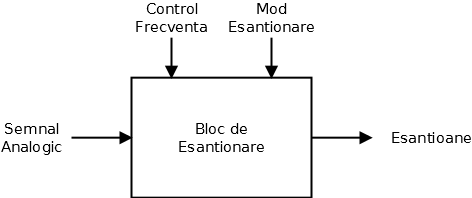
\includegraphics[width=220pt]{bloc_esantionare}
	\caption{Blocul de esantionare}
	\label{fig:bloc_esantionare}
\end{figure}		
		
	\item[a. Afisarea semnalului]		
		presupune reprezentarea esantioanelor prezente in memoria interna pe un ecran. Afisarea poate fi implementata independent de modulul de esantionare, comunicand cu acesta printr-o memorie de esantioane. Blocul de afisare va avea ca intrare memoria de esantionari, iar ca iesire un semnal VGA ce poate fi trimis catre orice monitor.
		
\begin{figure}[h]
	\centering
	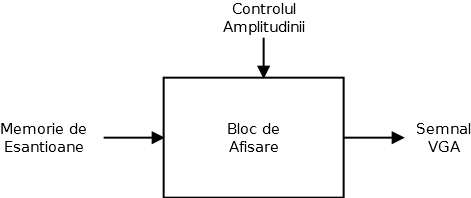
\includegraphics[width=240pt]{bloc_afisare}
	\caption{Blocul de afisare}
	\label{fig:bloc_afisare}
\end{figure}		
\end{description}

\paragraph{}
Cele doua blocuri vor fi implementate separat si vor comunica sincron printr-o memorie de esantioane. Aceasta memorie va contine suficiente esantioane ca sa se poata construi forma de unda pe ecran. Detaliile implementari pot fi gasite in sectiunea urmatoare a documentatiei.


\subsection{Continutul si Structura Documentului}
\paragraph{}
Acest document este impartit in sase sectiuni, fiecare completand si continuand sectiunea anterioara. Aceste sectiuni sunt:

% ---------------------------------------------------------
%	Continutul si Structura Documentului
% ---------------------------------------------------------
\renewcommand{\labelitemi}{$\bullet$}
\begin{description}

	\item[1. Rezumat]
		Aceasta sectiune contine o sinteza scurta a continutului intregului document. Aici sunt prezentate ideile principale din fiecare sectiunie care urmeaza.
		
	\item[2. Introducere] 
		Introducerea are rolul de a plasa problema proiectului in context, de a prezenta scopul proiectului si pozitia acestuia in domeniul studiat. Se analizeaza utilitatea proiectului luand in considerare constragerile platformei pe care este implementat si timpul de dezvoltare al acestuia.
		
	\item[3. Fundamente Teoretice]
		In sectiunea de fundamente teoretice sunt explicate notiunile de baza ale domeniului studiat (analiza semnalelor analogice periodice), implementari similare si o descriere a solutiei propuse. Sunt amintite referintele bibliografice din care s-au documentat autorii.
		
	\item[4. Proiectare si Implementare]
		Aceasta sectiune descrie pe larg structura si implementarea proiectului pe baza notiunilor teoretice prezentate anterior. Este prezentata platforma hardware folosita, impreuna cu deciziile pe care autorii le-au luat la implementarea proiectului.
		
	\item[5. Rezultate Experimetale]
		Aceasta sectiune are rolul de a demonstra corectitudinea implementarii prin exemplificarea functionalitatii. Sunt analizate rezultatele proiectului prin simulare asistata de calculator dar si prin implementarea si rularea sa pe suportul hardware.
		
	\item[6. Concluzii]
		Sectiunea de concluzii cuprinde propriile concluzii ale autorilor, experienta dobandita in urma implementarii proiectului dar si o analiza asupra procesului de implementare si produsul realizat.
		
\end{description}

% ---------------------------------------------------------

\clearpage